% Self-contained report. Compile with: pdflatex report.tex
% This is a paper section; the body lives directly in this file.

\documentclass[11pt,a4paper]{article}

\usepackage[margin=1in]{geometry}
\usepackage{amsmath}
\usepackage{amssymb}
\usepackage{booktabs}
\usepackage{siunitx}
\sisetup{detect-all=true}
% Atomic units removed from modern siunitx -- declare locally.
\DeclareSIUnit{\rydberg}{Ry}
\DeclareSIUnit{\bohr}{\ensuremath{a_{0}}}
\DeclareSIUnit{\bohrmagneton}{\ensuremath{\mu_{\mathrm{B}}}}
\usepackage{chemformula}
\usepackage{microtype}
\usepackage{enumitem}
\setlist{nosep}
\usepackage{xcolor}
\usepackage{graphicx}
\usepackage{subcaption}
\usepackage{hyperref}
\hypersetup{colorlinks=true, linkcolor=black, urlcolor=blue!60!black,
            citecolor=blue!60!black}

\title{DFT calculation}
\date{\today}

\begin{document}
\maketitle

\section{Destabilisation of \ch{MgH2} and \ch{Mg2NiH4} by substitutional
         Ni and Co dopants: a first-principles study}
\label{sec:nicodop}

Magnesium-based hydrides are leading materials for solid-state hydrogen
storage, with high gravimetric capacity and low cost. Pure \ch{MgH2} holds
\SI{7.6}{\percent} hydrogen by mass, but its large formation enthalpy
($\Delta H_\mathrm{f} = \SI{-74.5}{\kilo\joule\per\mol}~\ch{H2}$~\cite{bogdanovic1999,stampfer1960})
makes the hydride too stable for practical use, requiring dehydrogenation
near \SI{300}{\celsius}. The intermetallic \ch{Mg2Ni} forms a less stable
hydride, \ch{Mg2NiH4} ($\Delta H = \SI{-64.4}{\kilo\joule\per\mol}~\ch{H2}$~\cite{reilly1968}),
which desorbs more easily but stores less ($\sim$\SI{3.6}{\percent}). An effective additive
destabilises the hydride, raising $\Delta H$ toward zero and lowering the
desorption temperature.

We use density-functional theory (DFT) to compute the hydride formation
enthalpy for a single substitutional Ni or Co atom in each host, quantifying
the destabilisation produced by each dopant and, for Co in \ch{Mg2Ni}, its
dependence on the substitution site.

\subsection{Methods}
\label{sec:nicodop:methods}

We evaluate six hydrogenation reactions, three per host, on a common
per-\ch{H2} basis. For the \ch{Mg} host, reactant and product supercells have
identical metal content, so $\Delta H$ follows from the balanced reaction:
\begin{align}
\ch{Mg}        &+ \phantom{1}\ch{H2} \longrightarrow \ch{MgH2}        \tag{R1, pure}\\
\ch{Mg_{15}Ni} &+ 16\,\ch{H2}        \longrightarrow \ch{Mg_{15}NiH_{32}} \tag{R2, Ni 6.25\%}\\
\ch{Mg_{15}Co} &+ 16\,\ch{H2}        \longrightarrow \ch{Mg_{15}CoH_{32}} \tag{R3, Co 6.25\%}
\end{align}
The supercells are $2\!\times\!2\!\times\!2$ replications of rutile \ch{MgH2}
(product, 48 atoms) and hexagonal close-packed \ch{Mg} (reactant, 16 metal
sites), with one site replaced by the dopant: \SI{6.25}{at.\percent},
equivalent to \SI{13.87}{wt.\percent} (Ni) or \SI{13.92}{wt.\percent} (Co) of
the metal. All Mg sites are symmetry-equivalent, so the placement is unique.

For the \ch{Mg2Ni} host the pristine reaction uses the 18-atom hexagonal
\ch{Mg2Ni} cell and the 28-atom monoclinic ($C2/c$) \ch{Mg2NiH4} cell:
\begin{equation}
\tfrac{8}{12}\,\ch{Mg_{12}Ni6} + 8\,\ch{H2} \longrightarrow \ch{Mg8Ni4H16}.
\tag{R4, pure}
\end{equation}
The doped 18- and 28-atom cells differ in metal content, so doped enthalpies
use the dilute-defect limit,
\begin{equation}
\Delta\Delta H = \frac{1}{n_{\ch{H2}}}\bigl[(E_{\mathrm{hyd}}^{\,\mathrm{doped}}
 - E_{\mathrm{hyd}}^{\,\mathrm{pure}}) -
 (E_{\mathrm{met}}^{\,\mathrm{doped}} - E_{\mathrm{met}}^{\,\mathrm{pure}})\bigr]
 \times \SI{1312.75}{\kilo\joule\per\mol\per\rydberg},
\label{eq:defect}
\end{equation}
in which the Mg and dopant chemical potentials cancel. We treat Ni at an Mg
site (R5), Co at an Mg site (R6), and Co at a Ni site (R6$'$), the last
because Co favours the Ni site in \ch{Mg2Ni} ($E_{\mathrm{Mg}\to\mathrm{Ni}}
= \SI{-0.53}{eV}$~\cite{yoon2024}). Figures~\ref{fig:mg}
and~\ref{fig:mg2ni} show the relaxed product structures.

\begin{figure}[h!]
\centering
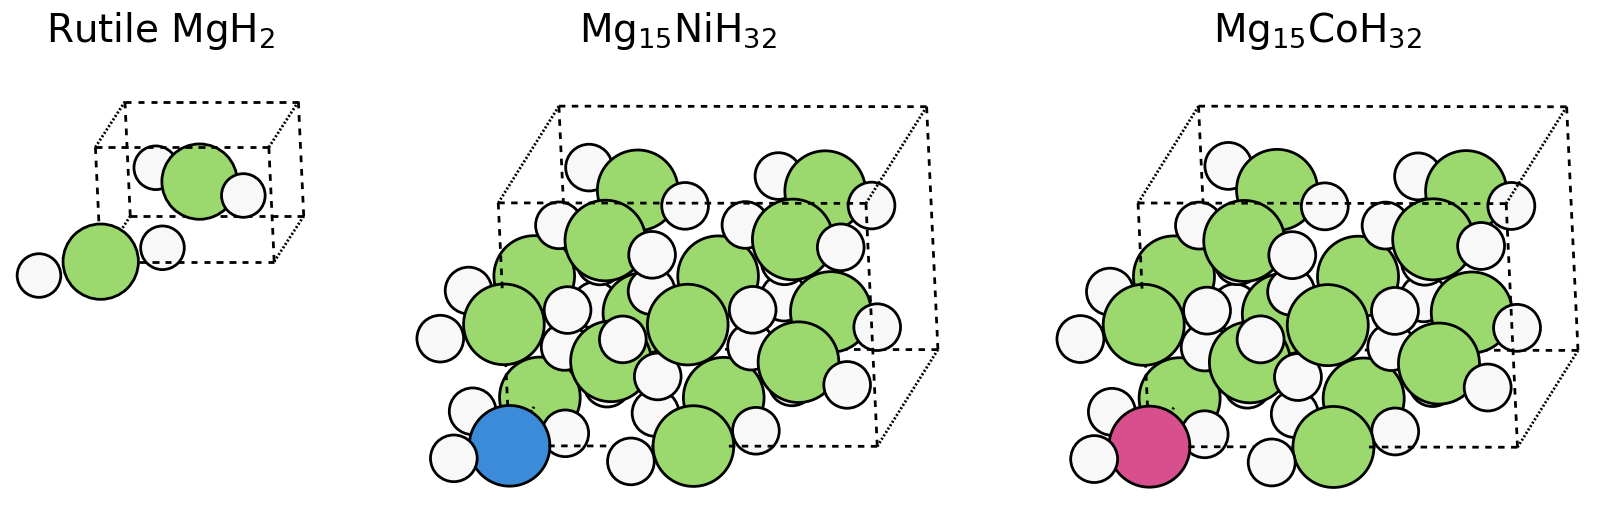
\includegraphics[width=\textwidth]{../figures/mg_host.png}
\caption{Relaxed product structures for the \ch{Mg} host: pristine rutile
\ch{MgH2} (left) and the Ni- and Co-substituted hydrides \ch{Mg_{15}NiH_{32}}
and \ch{Mg_{15}CoH_{32}} (right) at \SI{6.25}{at.\percent}. Atom colours: Mg
(green), H (white), Ni (blue), Co (pink).}
\label{fig:mg}
\end{figure}

\begin{figure}[h!]
\centering
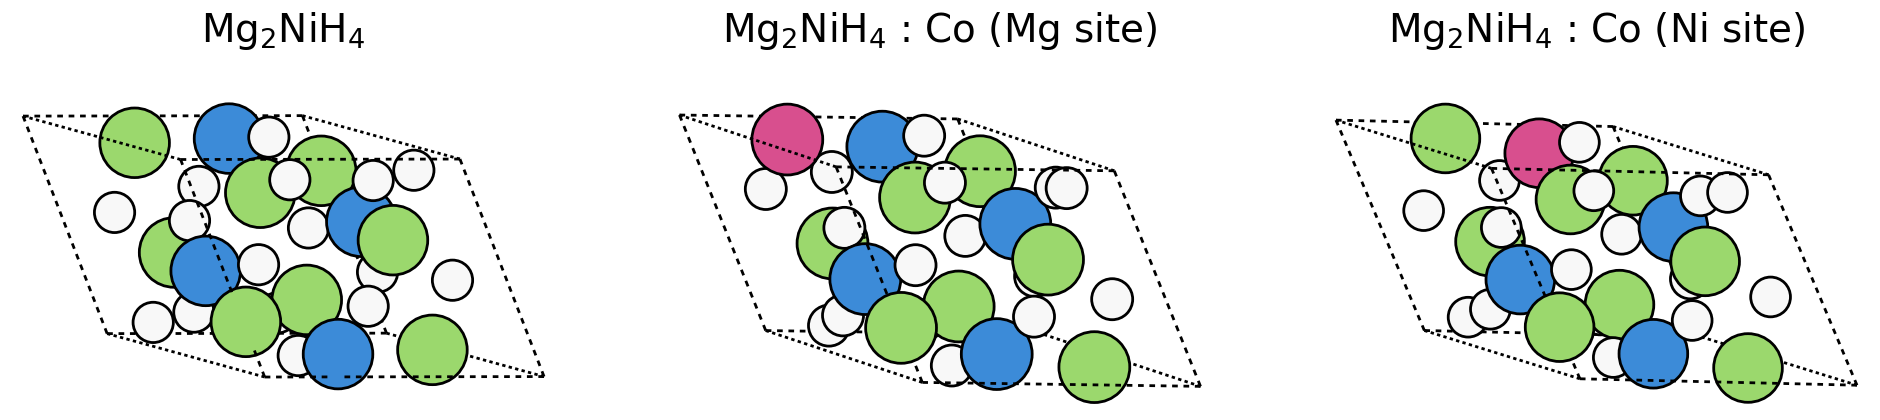
\includegraphics[width=\textwidth]{../figures/mg2ni_host.png}
\caption{Relaxed product structures for the \ch{Mg2Ni} host: pristine
\ch{Mg2NiH4} (left), and Co substituted at an Mg site (centre, R6) and at a
Ni site (right, R6$'$). Co favours the Ni site, where the destabilising
effect is negligible.}
\label{fig:mg2ni}
\end{figure}

All calculations use Quantum ESPRESSO~\cite{giannozzi2017} with the
Perdew--Burke--Ernzerhof (PBE) functional and Grimme-D3
dispersion~\cite{grimme2010}. Plane-wave cutoffs are \SI{60}{\rydberg}
(wavefunctions) and \SI{480}{\rydberg} (charge density); pseudopotentials are
projector augmented-wave for Mg and H, ultrasoft for Ni and Co.
Brillouin-zone integration uses $\Gamma$-centred grids at
$\sim$\SI{0.03}{\per\angstrom} ($12\!\times\!12\!\times\!8$ for the Mg
primitive cell, $8\!\times\!8\!\times\!12$ for rutile \ch{MgH2},
$6\!\times\!6\!\times\!4$ for the Mg supercell, $4\!\times\!4\!\times\!6$ for
the hydride supercell, $8\!\times\!8\!\times\!4$ for \ch{Mg2Ni}, and
$8\!\times\!8\!\times\!6$ for \ch{Mg2NiH4}). Metals use cold smearing
(\SI{0.01}{\rydberg}); the isolated \ch{H2} molecule uses fixed occupations.
The self-consistent field is converged to \SI{1e-9}{\rydberg}, and geometries
relaxed until forces fall below \SI{1e-4}{\rydberg\per\bohr}. No Hubbard $U$
is applied, so all six reactions share one energy scale. The formation
enthalpy per \ch{H2} is
\begin{equation}
\Delta H = \frac{1}{n_{\ch{H2}}}\,
   \bigl[\,E(\text{hydride}) - E(\text{metal}) - n_{\ch{H2}}\,E(\ch{H2})\bigr]
   \times \SI{1312.75}{\kilo\joule\per\mol\per\rydberg}.
\end{equation}

Each cell is evaluated in its electronic ground state, confirmed by
spin-polarised single-point calculations. Ni is nonmagnetic in every
environment; spin-polarised relaxation of the Ni-substituted metal gives zero
moment. Co carries an environment-dependent moment:
\SI{1.84}{\bohrmagneton} in \ch{Mg_{15}Co}, \SI{2.83}{\bohrmagneton} and
\SI{1.45}{\bohrmagneton} at the Mg and Ni sites of metallic \ch{Mg2Ni}, and
\SI{1.18}{\bohrmagneton} in \ch{Mg_{15}CoH_{32}}. It is quenched
($\le\!\SI{0.4}{\bohrmagneton}$) only at the hydrogen-coordinated sites of
\ch{Mg2NiH4}. Cells with a finite Co moment are relaxed spin-polarised. This
shifts $\Delta\Delta H$ from $+4.70$ to \SI{+4.09}{\kilo\joule\per\mol}
(\ch{Mg}:Co) and from $+13.28$ to \SI{+15.03}{\kilo\joule\per\mol}
(\ch{Mg2Ni}:Co, Mg site), without changing either sign.

\subsection{DFT results}
\label{sec:nicodop:results}

Table~\ref{tab:nicodop:dH} lists the formation enthalpies. Each dopant
destabilises both hosts at the Mg site: the four Mg-site $\Delta\Delta H$
values are positive and exceed the numerical uncertainty by an order of
magnitude. Ni is the stronger destabiliser ($\Delta\Delta H = +11.86$ and
\SI{+14.43}{\kilo\joule\per\mol}), and \ch{Mg}:Ni retains the full
\SI{7.1}{wt.\percent} capacity of magnesium.

\begin{table}[h!]
\centering
\sisetup{table-alignment-mode=format, table-number-alignment=right}
\begin{tabular}{l l S[table-format=-3.2] S[table-format=+2.2] c}
\toprule
& Pathway & {$\Delta H$ / kJ\,mol$^{-1}$\,\ch{H2}} & {$\Delta\Delta H$} & Effect \\
\midrule
R1   & pure \ch{Mg}              & -63.75 & {---}  & baseline \\
R2   & \ch{Mg} : Ni (6.25\%)     & -51.89 & +11.86 & destabilises \\
R3   & \ch{Mg} : Co (6.25\%)     & -59.66 &  +4.09 & destabilises \\
\midrule
R4   & pure \ch{Mg2Ni}           & -66.97 & {---}  & baseline \\
R5   & \ch{Mg2Ni} : Ni           & -52.54 & +14.43 & destabilises \\
R6   & \ch{Mg2Ni} : Co (Mg site) & -51.94 & +15.03 & destabilises \\
R6$'$& \ch{Mg2Ni} : Co (Ni site) & -68.71 &  -1.74 & $\approx$ neutral \\
\bottomrule
\end{tabular}
\caption{Hydrogenation enthalpy per absorbed \ch{H2} for the six pathways. A
less-negative $\Delta H$ (positive $\Delta\Delta H$) indicates a less stable
hydride, which is easier to dehydrogenate. $\Delta\Delta H$ is referenced to
the corresponding pure host (R1 for the \ch{Mg} host, R4 for the \ch{Mg2Ni}
host).}
\label{tab:nicodop:dH}
\end{table}

The exception is Co at its preferred Ni site (R6$'$), which is marginally
stabilising ($\Delta\Delta H = \SI{-1.74}{\kilo\joule\per\mol}$). This is an
order of magnitude smaller than the Mg-site shifts, comparable to the
$\sim$\SI{1.4}{\kilo\joule\per\mol} variation across the three inequivalent
Mg sites of \ch{Mg2NiH4}~\cite{yoon2024}, and well below the
$\sim$\SI{10}{\kilo\joule\per\mol} zero-point correction, so Co at the Ni
site is effectively inert. The benefit of Co in \ch{Mg2Ni} thus depends on
site occupancy: the Mg site destabilises strongly, as in non-equilibrium
ball-milled material, while the equilibrium Ni site does not.

The pure-\ch{Mg} baseline ($\Delta H =
\SI{-63.75}{\kilo\joule\per\mol}~\ch{H2}$) lies $\sim$\SI{11}{\kilo\joule
\per\mol} above experiment, reflecting the known GGA under-binding of ionic
\ch{MgH2} (Er et al.\ obtain \SI{-63.7}{\kilo\joule\per\mol} with
PW91~\cite{er2009}; Pozzo and Alf\`e require quantum Monte Carlo to match
experiment~\cite{pozzo2008}). The pure-\ch{Mg2Ni} baseline
($\SI{-66.97}{\kilo\joule\per\mol}$) agrees with experiment~\cite{reilly1968}
to within \SI{2.6}{\kilo\joule\per\mol}; the hydrogen in \ch{Mg2NiH4} forms
covalent \ch{[NiH4]^{4-}} complexes~\cite{yoon2024} that the GGA describes
more accurately than the ionic \ch{H^-} of \ch{MgH2}. This host-dependent error
($\sim$\SI{13}{\kilo\joule\per\mol}) prevents the absolute enthalpies from
reproducing the experimental host ordering, so we draw no cross-host
conclusions from absolute values. The within-host differences $\Delta\Delta
H$ cancel this error and are robust; the same cancellation underlies the GGA
survey of Yoon et al.~\cite{yoon2024}, whose relative predictions reproduce
plateau-pressure trends for seven solutes in \ch{MgH2} and ten in
\ch{Mg2Ni}. For an absolute estimate, the shift can be referenced to the
experimental host enthalpy, $\Delta H \approx \Delta H_{\exp} + \Delta\Delta
H_{\mathrm{DFT}}$, giving \SI{-62.6}{\kilo\joule\per\mol} for \ch{Mg}:Ni and
\SI{-50.0}{\kilo\joule\per\mol} for \ch{Mg2Ni}:Ni, with estimated 1-bar
desorption temperatures of \SI{207}{\celsius} and \SI{110}{\celsius}
(van~'t~Hoff, $\Delta S = \SI{130.5}{\joule\per\mol\per\kelvin}$).

A single Ni or Co atom at an Mg site destabilises both \ch{MgH2} and
\ch{Mg2NiH4}, lowering the thermodynamic barrier to hydrogen release. Ni
is the stronger, more reliable catalyst for both hosts, and \ch{Mg}:Ni
preserves the high capacity of magnesium. Co is effective in \ch{Mg} and
at the Mg site of \ch{Mg2Ni}, but inert at its preferred Ni site. These
results give a thermodynamic basis for the improved dehydrogenation of Ni-
and Co-doped magnesium hydrides. Two limitations apply: the calculations
address thermodynamics only, not the activation barriers behind the
additives' kinetic role; and zero-point energy, omitted here, amounts to
$\sim$\SI{15}{\kilo\joule\per\mol}~\ch{H2} for these hydrides~\cite{er2009}
but, being similar for doped and pure cells, largely cancels in
$\Delta\Delta H$.

\bibliographystyle{unsrt}
\bibliography{refs}

\end{document}
